\documentclass{article}

% --- load packages ---

\usepackage[margin=1in]{geometry} % change the margins
\usepackage{amsmath} % useful math environments and commands like align
\usepackage{amssymb} % assumes amsmath package installed
\usepackage[colorlinks,bookmarks,bookmarksnumbered,allcolors=blue]{hyperref} % hyperlinks between references
\usepackage{graphicx}  % include images
\usepackage[caption=false]{subfig} % subfigures.  false option prevents conflicts in caption styling with other packages
\usepackage{booktabs} % better tables
\usepackage[capitalise]{cleveref} % better referencing. uses cref.
\usepackage[section]{placeins} % sometimes useful to prevent figures from floating out of a section
\usepackage{cite} % handles multiple citations in one command better
\usepackage{doi} % allow correct hypderlinking of DOIs
\usepackage{hyperref}
\usepackage[title]{appendix}
\usepackage{pgfplots}
\usepackage{algorithm} % for algorithm figure
\usepackage{algpseudocode} % for algorithm figure

\usepackage{aircraftshapes}

\newcommand{\norm}[1]{\left\Vert{#1}\right\Vert}
\newcommand{\skewm}[1]{\left[{#1}\right]_{\times}}


\begin{document}

\title{Homework 6}
\author{Jaron Ellingson}
% put in \date{} if you don't want a date to appear, or enter a specific date, otherwise default is today's date.
\maketitle

 %\href{https://byu.box.com/shared/static/anxheci3eytucrh3ke57k2sqdx0ivmjg.pdf}{homework pdf}

\section*{6.1 Project Update}

For my final project I have been busy putting all the pieces together to allow for real-time control of a fixed-wing aircraft using an evolutionary based model predictive control algorithm. We choose to implement this method using nonlinear dynamics which is a little harder to solve than using linearized dynamics. However, we have been able to speed up our evolutionary algorithm and have perform the optimization real time. \Cref{fig:results} shows the positional states for the fixed-wing when commanded to follow a circular trajectory and maintain a certain height.  \Cref{fig:inputs_results} shows the inputs to the system which appear to less jumpy than previous attempts and indicate that the aircraft is choosing values which will provide some stability to the system. While we are excited about these results we want to improve these results to be better following the trajectory path.

\begin{figure}[htbp]
	\centering
	\subfloat[]{
		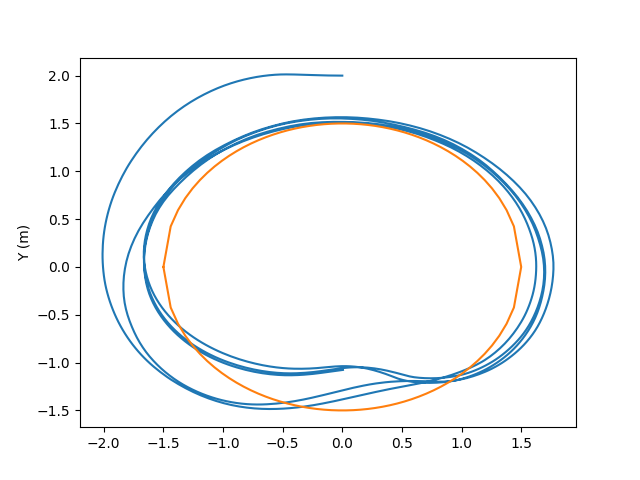
\includegraphics[width=0.45\textwidth]{figures/XY.png}
		\label{fig:xy}
	}
	\qquad
	\subfloat[]{
		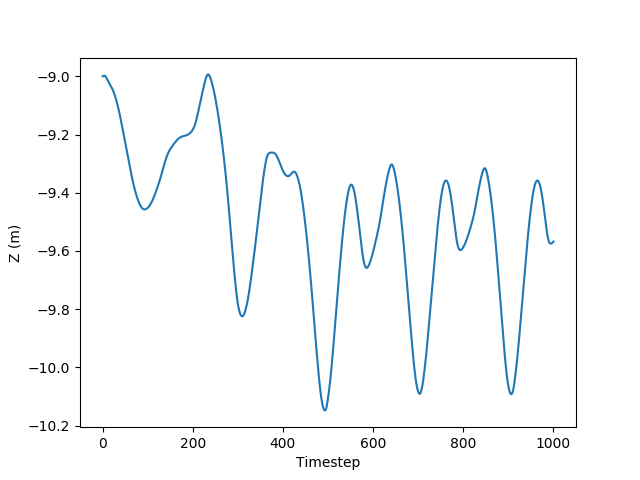
\includegraphics[width=0.45\textwidth]{figures/Z.png}
		\label{fig:z}
	}
	\caption{The positional states for a fixed-wing aircraft following a circular trajectory. The orange is the commanded state while the blue is the actual state. \Cref{fig:xy} compares the x and y states while \Cref{fig:z} compares only the z state.}
	\label{fig:results}
\end{figure}

\begin{figure}[htbp]
	\centering
	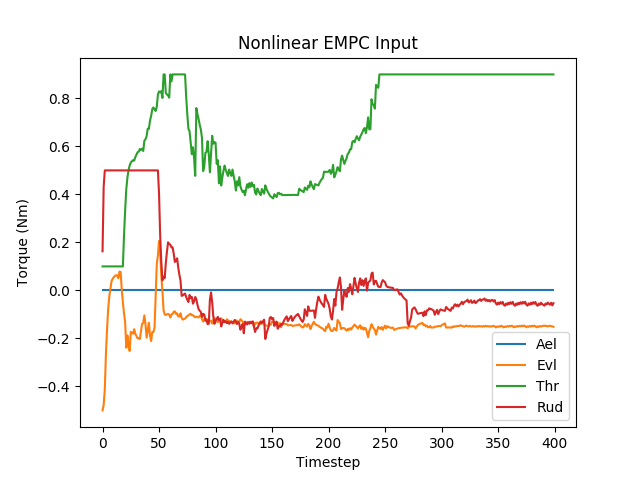
\includegraphics[width=0.45\textwidth]{figures/inputs.png}
	\caption{The inputs chosen for the trajectory.}
	\label{fig:inputs_results}
\end{figure}

\section*{6.2 Optimization Under Uncertainty}

For optimization under uncertainty portion of this homework, we implemented statistical convergence for a wind farm minimizing cost of energy (COE). We first sampled the three parameter distributions and created the output distribution with these parameters. \Cref{fig:convergence} shows that the 95th percentile converges to around 3200 samples for this particular problem. Finally, minimized the 95th percentile of the COE output with 3200 samples. \Cref{tab:comp_der} shows the comparison of the deterministic COE and the 95th percentile COE optimizations. If we were to only use the deterministic optimizations then we would have roughly a 5\% decrease in accuracy at a 95th percentile. Overall, I learned the uncertainty optimization is very important and will lead to designs which are safe and robust.



\begin{figure}[htbp]
	\centering
	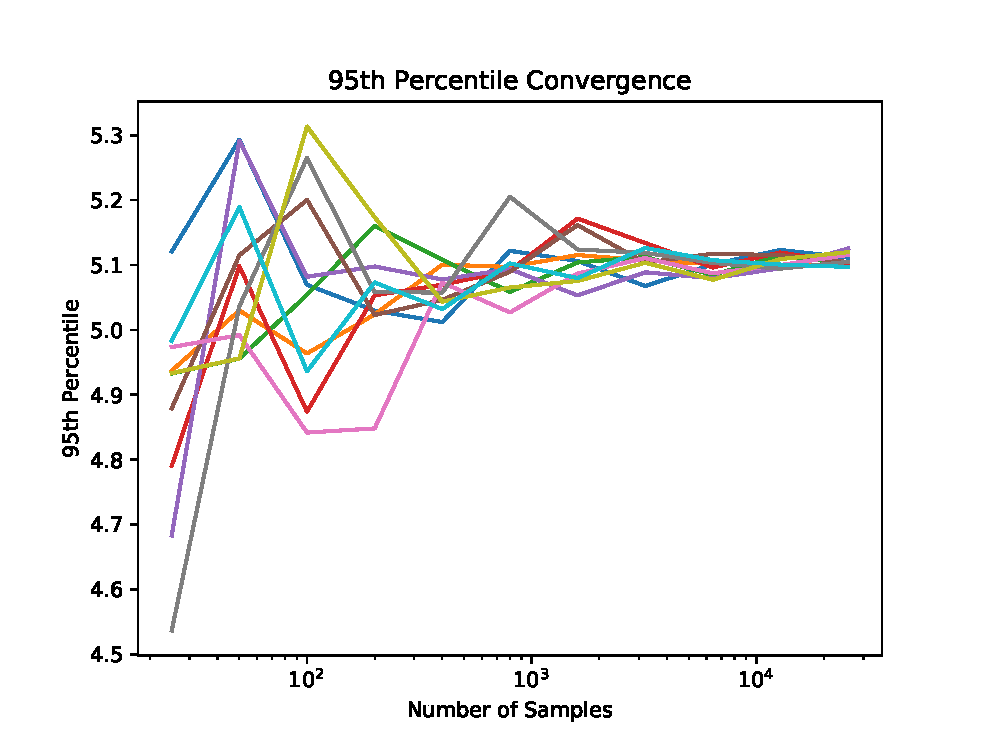
\includegraphics[width=0.45\textwidth]{figures/convergence.eps}
	\caption{Convergence plot of several different sample sizes over many different trials. The 95th percentile appears to converge around 3200 samples.}
	\label{fig:convergence}
\end{figure}


 
\begin{table}[htb]
	\centering
	\caption{We measured convergence efficiency of the four mentioned algorithms through comparing solve time, total trajectory error, and final state error.}
	\label{tab:comp_der}
	\begin{tabular}{c|c|c}
		\toprule
		Layout & Deterministic COE & 95th Percentile COE \\
		\midrule
		Deterministic Layout & 2.1845 & 2.3716 \\
		OUU Layout & 2.2340 & 2.2542 \\
		\bottomrule
	\end{tabular}
\end{table}


\section*{6.3 Surrogate-Base Optimization}

The final section of this homework was the surrogate-based optimization of supersonic body of revolution. This problem required using a optimization function which was similar to a computational fluid dynamics (CFD) simulation. This made solving this problem very slow and so we used a surrogate-model approach. We first knew roughly the shape of the solution and so we choose a shape for the surrogate without using the cross-validation approach. We sampled the design space using latin-hypercube sampling and then used the exploitation model for infilling the surrogate. This led the the result shown in \Cref{fig:sur_model} that shows the surrogate model finding a solution which is very close the the Sears-Haack theoretical solution.

\begin{figure}[htbp]
	\centering
	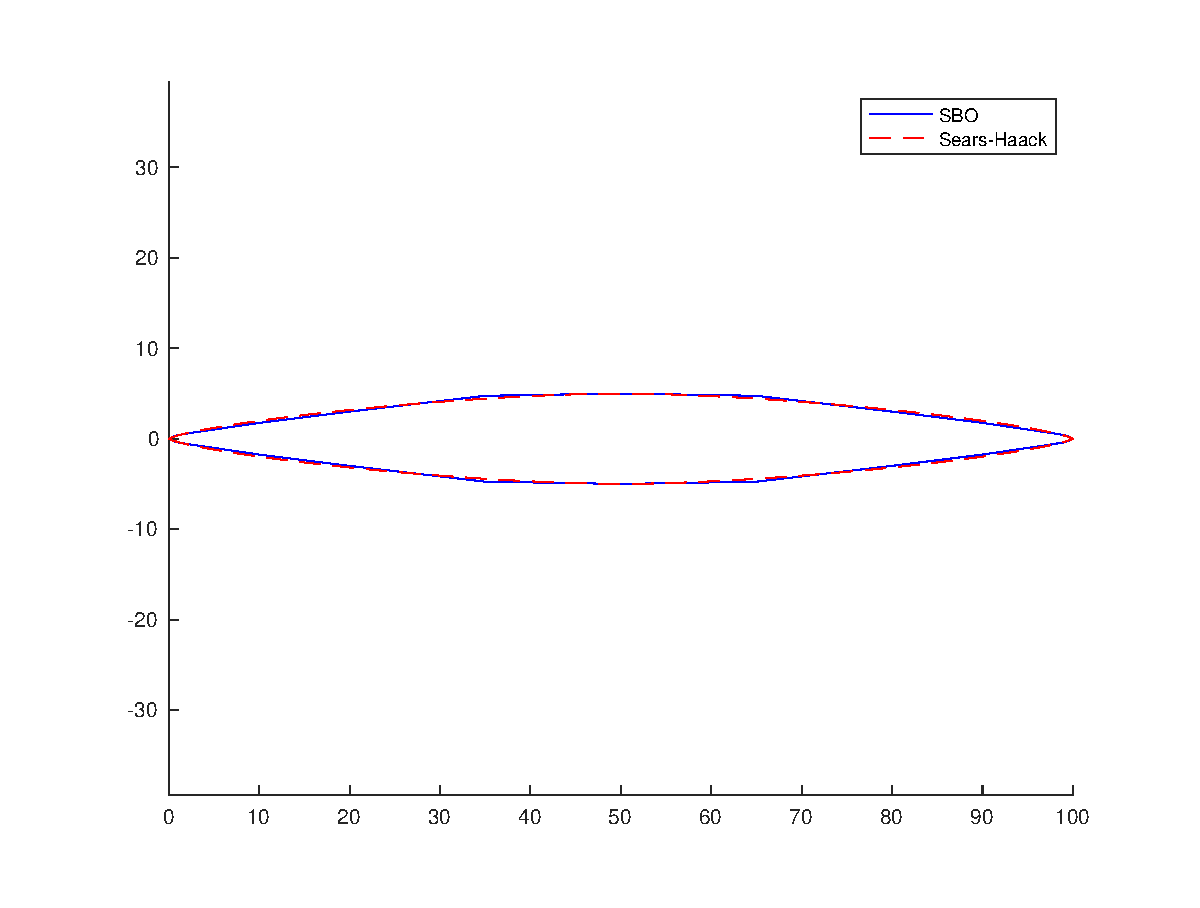
\includegraphics[width=0.45\textwidth]{figures/surrogate_modeling.eps}
	\caption{Surrogate model verses the theoretical solution.}
	\label{fig:sur_model}
\end{figure}

Overall, I learned the surrogate-modeling can yield good results and is an attractive method to use when the function evaluations take an unrealistic amount of time.


\bibliographystyle{unsrt}
\bibliography{references}


\end{document}